% =====================================================================
%  Guía de laboratorio — IEL04 — Circuitos Eléctricos I, semana 9
%  Escrita por src/guia_laboratorio.py con la plantilla institucional
%  (config/framework_iub/guia-laboratorio/: guialabiub.sty e img/, copiados a esta carpeta).
%
%  Compilar con:  pdflatex -> biber -> pdflatex -> pdflatex
%  (En Overleaf: compilador pdfLaTeX; biber se ejecuta solo.)
% =====================================================================
\documentclass[12pt]{article}

% Opciones: [sinmarca] quita la marca de agua; [borrador] muestra márgenes
%           [ieee] referencias IEEE (por defecto); [apa] referencias APA 7
\usepackage{guialabiub}

% ------- Tablas, diagramas de flujo, circuitos y gráficas (todo en LaTeX) -------
% (la plantilla no los trae; los estilos y la paleta son los del .tex del temario)
\usepackage{colortbl}                    % encabezado #121023 y filas alternas en las tablas
\usepackage{xltabular}                   % la tabla de materiales se parte entre páginas
\usepackage{tikz}
\usetikzlibrary{arrows.meta,positioning,shapes.geometric,shapes.misc}
\usepackage[siunitx,RPvoltages]{circuitikz}
\usepackage{pgfplots}
\pgfplotsset{compat=1.18}
\usepackage{adjustbox}

% Paleta del Manual de Identidad Visual IUB 2025 (los colores del manual y sus tintes)
\definecolor{iubnavy}{HTML}{121023}
\definecolor{iubyellow}{HTML}{FFDF2D}
\definecolor{iubwhite}{HTML}{FFFFFF}
\definecolor{iubblue}{HTML}{00ADE7}
\definecolor{iuborange}{HTML}{E39037}
\definecolor{iubgreen}{HTML}{3B9C6D}
\colorlet{iubgris}{iubnavy!18}
\colorlet{iubgrisoscuro}{iubnavy!60}
\colorlet{iubfondoazul}{iubblue!8}
\colorlet{iubfondonaranja}{iuborange!10}
\colorlet{iubfondoverde}{iubgreen!9}
\colorlet{iubfondogris}{iubnavy!5}
\colorlet{iubpurple}{iubnavy!45}
\pgfplotsset{cycle list={{iubblue, mark=*},{iuborange, mark=square*},{iubgreen, mark=triangle*},{iubnavy, mark=diamond*},{iubyellow, mark=pentagon*}}}

% Estilos de los diagramas de flujo (TikZ) y de las gráficas (pgfplots)
\tikzset{
  dcaja/.style={draw=iubblue, fill=iubfondoazul, line width=1pt, rounded corners=1pt, align=center, inner sep=2pt, text=iubnavy},
  destado/.style={draw=iubblue, fill=iubfondoazul, line width=1pt, rounded corners=6pt, align=center, inner sep=2pt, text=iubnavy},
  ddecision/.style={draw=iuborange, fill=iubfondonaranja, line width=1pt, diamond, aspect=1.6, align=center, inner sep=1pt, text=iubnavy},
  dterminal/.style={draw=iubgreen, fill=iubfondoverde, line width=1pt, rounded rectangle, align=center, inner sep=2pt, text=iubnavy},
  dflecha/.style={-{Stealth[length=2.4mm]}, line width=0.9pt, draw=iubnavy},
  drotulo/.style={font=\footnotesize, text=iubgrisoscuro, fill=white, fill opacity=0.92, text opacity=1, inner sep=1.5pt},
}
\pgfplotsset{iubejes/.style={width=0.9\linewidth, height=6.2cm, grid=major, grid style={iubgris}, axis lines*=left, axis line style={iubnavy}, tick label style={font=\small}, label style={font=\small}, title style={font=\bfseries\small}, legend cell align=left, legend style={draw=none, fill=none, font=\small, anchor=north, legend columns=-1, /tikz/every even column/.append style={column sep=8pt}}, unbounded coords=jump}}

% --------------------------- Bibliografía ----------------------------
\addbibresource{IEL04-semana09.bib}

% --------------------------- Datos de la guía -------------------------
\facultad{Facultad de Ingenierías}
\modulo{IEL04 --- Circuitos Eléctricos I}
\docente{Ing. Sergio Martinez Castilla}

\begin{document}

% Orden de la bibliografía: el mismo del .md (biblatex numera por orden de primera cita)
\nocite{ref1,ref2,ref3}

\datosguia
\lineablanco

% Título de la práctica y ficha de la sesión
{\centering\bfseries Guía de laboratorio: Identificación de una bobina por su constante de tiempo y su impedancia, y medición de un circuito RL mixto\par}
\lineablanco
\textbf{Semana:} 9 de 14 \quad \textbf{Resultado de aprendizaje:} IEL04-RA3 \quad \textbf{Práctica:} propuesta a partir de la bibliografía \cite{ref1}, \cite{ref2}, \cite{ref3} \quad \textbf{Duración:} \SI{240}{\minute}
\lineablanco
La práctica cierra el RA IEL04-RA3 y corresponde a la sesión teórica de la semana 9, \guillemotleft{}Cálculo y medición de parámetros en circuitos RL según el conexionado\guillemotright{}. Reproduce su caso de estudio: determinar la inductancia de una bobina sin marcado por dos métodos independientes ---su constante de tiempo con una onda cuadrada y su impedancia con una señal sinusoidal---, identificar a qué valor estándar corresponde y usarla en un circuito RL mixto, del que se miden la corriente, las tensiones y el factor de potencia. No hay un manual de laboratorio asignado, por lo que la práctica se propone a partir de la bibliografía cargada: Floyd trata la constante de tiempo L/R, la potencia en circuitos RL y los circuitos RL en serie-paralelo \cite{ref1}, Boylestad los transitorios R-L y los valores estándar de inductores \cite{ref2} y Deorsola el régimen transitorio del circuito RL \cite{ref3}.

% ---------------------------------------------------------------------
\section{Objetivos}\label{sec:objetivos}
\textbf{Objetivo general:} Determinar experimentalmente la inductancia de una bobina por dos métodos y verificar el cálculo de un circuito RL mixto.
\lineablanco
\textbf{Objetivos específicos:}
\begin{itemize}
  \item Identificar el valor estándar de una bobina sin marcado a partir de sus mediciones. \emph{(CE1)}
  \item Medir la constante de tiempo y la impedancia de la bobina en un circuito resistivo e inductivo. \emph{(CE2)}
  \item Medir corrientes, tensiones, ángulo y factor de potencia en un circuito RL mixto y compararlos con el cálculo. \emph{(CE3)}
\end{itemize}

% ---------------------------------------------------------------------
\section{Materiales y Equipos}\label{sec:materiales}
% --- Tabla: materiales y equipos (11; xltabular repite el encabezado si se parte) ---
\arrayrulecolor{iubnavy}
\begin{xltabular}{\linewidth}{>{\raggedleft\arraybackslash}p{0.6cm} >{\raggedright\arraybackslash}X >{\raggedright\arraybackslash}X >{\raggedleft\arraybackslash}p{2.2cm}}
\caption{Materiales y equipos de la práctica}\label{tab:materiales} \\
\rowcolor{iubnavy} \textcolor{white}{\textbf{\#}} & \textcolor{white}{\textbf{Material o equipo}} & \textcolor{white}{\textbf{Especificación}} & \textcolor{white}{\textbf{Cantidad}} \\
\endfirsthead
\rowcolor{iubnavy} \textcolor{white}{\textbf{\#}} & \textcolor{white}{\textbf{Material o equipo}} & \textcolor{white}{\textbf{Especificación}} & \textcolor{white}{\textbf{Cantidad}} \\
\endhead
\bottomrule
\endlastfoot
  1 & Bobina toroidal sin marcado & --- & 1 \\
  \rowcolor{iubfondogris} 2 & Resistor & 1 k\ensuremath{\Omega} (medido 996 \ensuremath{\Omega} en la sesión) & 1 \\
  3 & Resistor R1 & 470 \ensuremath{\Omega} & 1 \\
  \rowcolor{iubfondogris} 4 & Resistor R2 & 680 \ensuremath{\Omega} & 1 \\
  5 & Resistor sensor de corriente & 10 \ensuremath{\Omega} & 1 \\
  \rowcolor{iubfondogris} 6 & Generador de funciones & --- & 1 \\
  7 & Osciloscopio de dos canales con puntas \texttimes{}10 & --- & 1 \\
  \rowcolor{iubfondogris} 8 & Multímetro digital de verdadero valor eficaz & --- & 2 \\
  9 & Medidor LCR & --- & 1 \\
  \rowcolor{iubfondogris} 10 & Protoboard & --- & 1 \\
  11 & Cables de conexión & --- & 12 \\
\end{xltabular}

% ---------------------------------------------------------------------
\section{Procedimiento}\label{sec:procedimiento}
La práctica ocupa el bloque de 2 h de laboratorio de la sesión y se realiza en grupos de tres estudiantes, con tres roles que rotan entre etapas: quien monta y opera el circuito, quien mide y quien registra y verifica los cálculos. Antes de energizar cualquier montaje, el docente o el monitor revisa la conexión. Cada etapa abre con su diagrama de flujo, que muestra la secuencia y las comprobaciones de un vistazo, y sigue con sus pasos numerados; cada paso indica cuánto dura, qué debe observarse para saber que salió bien y qué hacer si no. Los valores numéricos de la sesión teórica sirven de referencia: las lecturas propias del grupo se registran en las tablas de la sección de análisis.
\lineablanco
% --- Etapa 1: Método 1: constante de tiempo (3 pasos) ---
\subsection{Método 1: constante de tiempo (\SI{21}{\minute})}\label{sec:etapa-1}
% --- Figura 1: diagrama de flujo de la etapa 1 (TikZ, con la paleta IUB) ---
\begin{figure}[H]
  \centering
\begin{adjustbox}{max width=\linewidth}
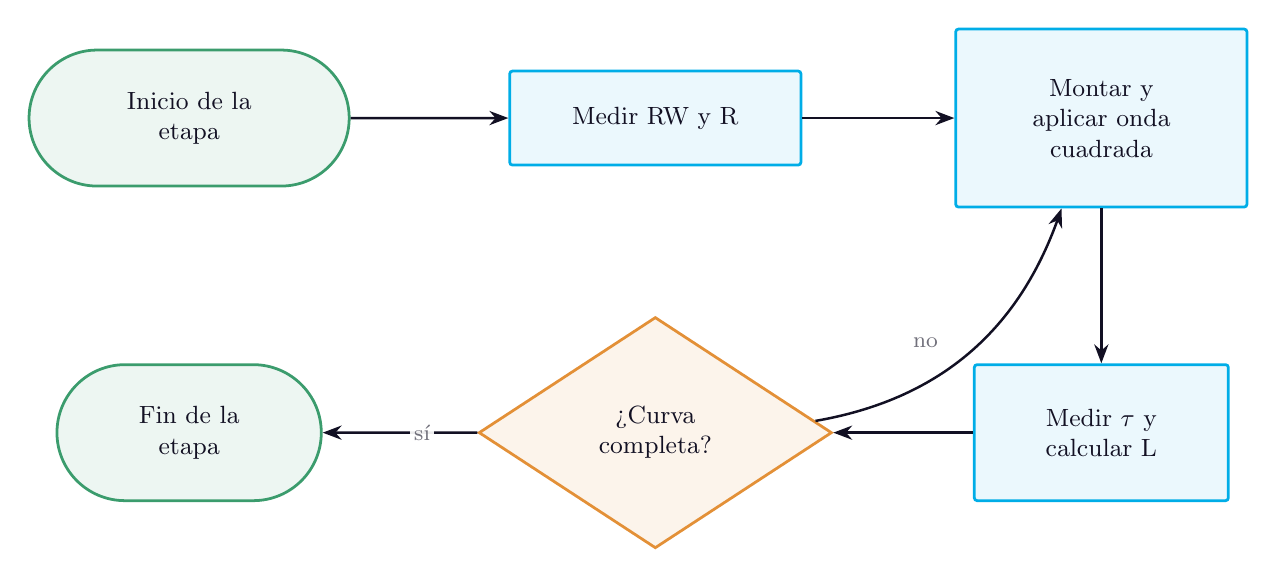
\begin{tikzpicture}[x=1in, y=1in, font=\small]
  % nodos (centro en pulgadas, con el tamano que calcula figuras.py)
  \node[dterminal, minimum width=1.656in, minimum height=0.680in] (n0) at (0.828,-0.445) {Inicio de la \\ etapa};  % ini
  \node[dcaja, minimum width=1.456in, minimum height=0.470in] (n1) at (3.159,-0.445) {Medir RW y R};  % a0
  \node[dcaja, minimum width=1.456in, minimum height=0.890in] (n2) at (5.389,-0.445) {Montar y \\ aplicar onda \\ cuadrada};  % a1
  \node[dcaja, minimum width=1.270in, minimum height=0.680in] (n3) at (5.389,-2.018) {Medir \ensuremath{\tau} y \\ calcular L};  % a2
  \node[ddecision, minimum width=1.766in, minimum height=1.156in] (n4) at (3.159,-2.018) {\textquestiondown{}Curva \\ completa?};  % dec
  \node[dterminal, minimum width=1.377in, minimum height=0.680in] (n5) at (0.828,-2.018) {Fin de la \\ etapa};  % fin
  % flechas (las de retorno, curvas)
  \draw[dflecha] (n0) -- (n1);
  \draw[dflecha] (n1) -- (n2);
  \draw[dflecha] (n2) -- (n3);
  \draw[dflecha] (n3) -- (n4);
  \draw[dflecha] (n4) -- (n5);
  \draw[dflecha] (n4) to[bend right=31] (n2);
  % rotulos de las flechas (donde no caen sobre un nodo)
  \node[drotulo] at (1.993,-2.018) {sí};
  \node[drotulo] at (4.510,-1.566) {no};
\end{tikzpicture}
\end{adjustbox}
  \caption{Diagrama de flujo de la etapa 1: Método 1: constante de tiempo}
  \label{fig:flujo-1}
\end{figure}
\begin{pasos}
  \item \textbf{Paso~1:} Medir con el ohmímetro la resistencia de devanado de la bobina y la del resistor de 1 k\ensuremath{\Omega}. \emph{(aprox.~\SI{5}{\minute})} \textbf{Comprobación:} La resistencia de devanado debe ser de pocos ohmios; una lectura infinita indica devanado abierto.
  \item \textbf{Paso~2:} Montar la bobina en serie con el resistor de 1 k\ensuremath{\Omega} y aplicar una onda cuadrada de 0 V a 5 V y 10 kHz. \emph{(aprox.~\SI{6}{\minute})} \textbf{Comprobación:} El docente revisa el montaje antes de energizar. \textbf{Seguridad:} Montar con el generador apagado.
% figura del paso 2: Medición de la constante de tiempo: bobina en serie con el resistor y el canal 2 sobre el… (circuito en circuitikz)
\par\medskip\noindent
\begin{minipage}{\linewidth}
  \centering
  \begin{adjustbox}{max width=\linewidth}
    \begin{circuitikz}[color=iubnavy]
    \draw (0,0) to[V, l=$v_s$] (0,3) to[L, l=$L$] (4,3) to[R, l=$R$] (4,0) -- (0,0); \draw (4,3) -- (6,3) to[voltmeter, l=CH2] (6,0) -- (4,0); \draw (0,0) node[ground]{};
    \end{circuitikz}
  \end{adjustbox}
  \captionof{figure}{Medición de la constante de tiempo: bobina en serie con el resistor y el canal 2 sobre el resistor}\label{fig:paso-2}
\end{minipage}
\par\medskip
  \item \textbf{Paso~3:} Con la punta del canal 2 sobre el resistor, medir con los cursores el tiempo en que la tensión alcanza el 63 \% de su valor final y calcular $L = \tau (R + R_W)$ \cite{ref1}. \emph{(aprox.~\SI{10}{\minute})} \textbf{Comprobación:} El semiperiodo de 50 \textmu{}s debe superar con holgura cinco constantes de tiempo; si la curva no llega a la meseta, reducir la frecuencia.
% ecuación del paso 3: Inductancia a partir de la constante de tiempo:
\par Inductancia a partir de la constante de tiempo:
\begin{equation}
  L = \tau \,(R + R_W)
  \label{eq:paso-3}
\end{equation}
donde $L$ en henrios (H), $\tau$ en segundos (s), $R$ y $R_W$ en ohmios (\ensuremath{\Omega}).
\end{pasos}
% --- Etapa 2: Método 2: impedancia (3 pasos) ---
\subsection{Método 2: impedancia (\SI{26}{\minute})}\label{sec:etapa-2}
% --- Figura 3: diagrama de flujo de la etapa 2 (TikZ, con la paleta IUB) ---
\begin{figure}[H]
  \centering
\begin{adjustbox}{max width=\linewidth}
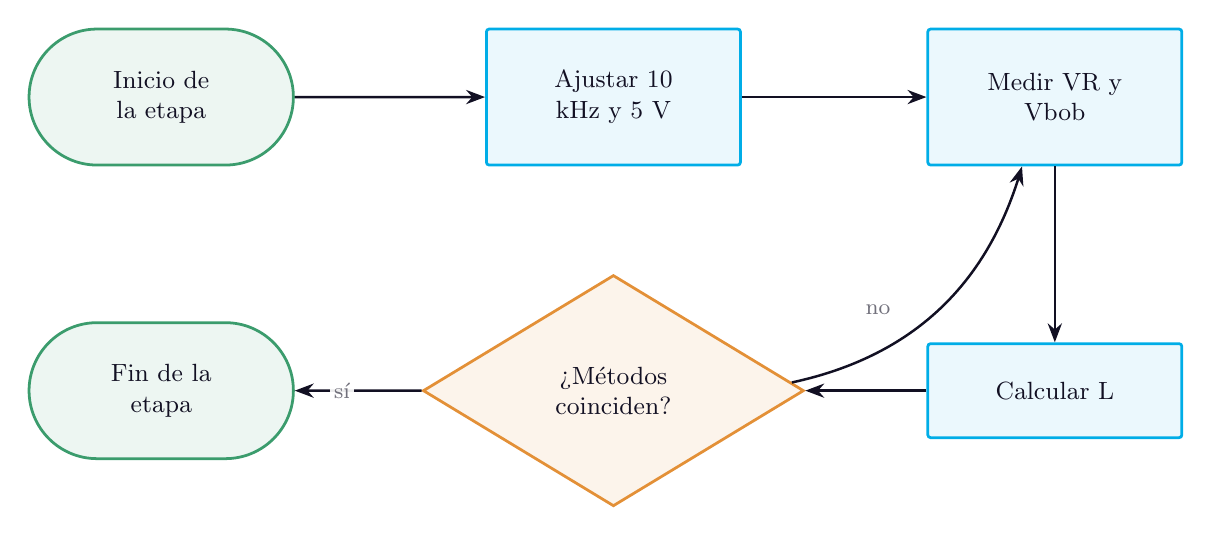
\begin{tikzpicture}[x=1in, y=1in, font=\small]
  % nodos (centro en pulgadas, con el tamano que calcula figuras.py)
  \node[dterminal, minimum width=1.377in, minimum height=0.680in] (n0) at (0.689,-0.340) {Inicio de \\ la etapa};  % ini
  \node[dcaja, minimum width=1.270in, minimum height=0.680in] (n1) at (2.950,-0.340) {Ajustar 10 \\ kHz y 5 V};  % a0
  \node[dcaja, minimum width=1.270in, minimum height=0.680in] (n2) at (5.157,-0.340) {Medir VR y \\ Vbob};  % a1
  \node[dcaja, minimum width=1.270in, minimum height=0.470in] (n3) at (5.157,-1.808) {Calcular L};  % a2
  \node[ddecision, minimum width=1.905in, minimum height=1.156in] (n4) at (2.950,-1.808) {\textquestiondown{}Métodos \\ coinciden?};  % dec
  \node[dterminal, minimum width=1.377in, minimum height=0.680in] (n5) at (0.689,-1.808) {Fin de la \\ etapa};  % fin
  % flechas (las de retorno, curvas)
  \draw[dflecha] (n0) -- (n1);
  \draw[dflecha] (n1) -- (n2);
  \draw[dflecha] (n2) -- (n3);
  \draw[dflecha] (n3) -- (n4);
  \draw[dflecha] (n4) -- (n5);
  \draw[dflecha] (n4) to[bend right=31] (n2);
  % rotulos de las flechas (donde no caen sobre un nodo)
  \node[drotulo] at (1.593,-1.808) {sí};
  \node[drotulo] at (4.273,-1.405) {no};
\end{tikzpicture}
\end{adjustbox}
  \caption{Diagrama de flujo de la etapa 2: Método 2: impedancia}
  \label{fig:flujo-2}
\end{figure}
\begin{pasos}
  \item \textbf{Paso~4:} Ajustar el generador a una onda sinusoidal de 10 kHz y medir con el osciloscopio y con el multímetro de verdadero valor eficaz que la tensión en los bornes del circuito, con el circuito conectado, sea de 5,00 V eficaces. \emph{(aprox.~\SI{6}{\minute})} \textbf{Comprobación:} El multímetro debe indicar 5,00 V y el osciloscopio una sinusoide sin distorsión; si la tensión baja al conectar el circuito, reajustar la amplitud con el circuito conectado.
  \item \textbf{Paso~5:} Medir la tensión en el resistor para obtener la corriente y la tensión en la bobina con la resta de canales del osciloscopio. \emph{(aprox.~\SI{10}{\minute})} \textbf{Comprobación:} Debe obtenerse una corriente cercana a 4,86 mA; si la resta de canales da ruido, verificar que ambos canales tengan la misma escala.
  \item \textbf{Paso~6:} Calcular $Z_{\mathrm{bob}} = V_{\mathrm{bob}}/I$, $X_L = \sqrt{Z_{\mathrm{bob}}^2 - R_W^2}$ y $L = X_L/(2\pi f)$, y compararla con la del método 1; identificar el valor estándar más cercano \cite{ref2}. \emph{(aprox.~\SI{10}{\minute})} \textbf{Comprobación:} Los dos métodos deben coincidir a pocos por ciento; si no, repetir la medición de \ensuremath{\tau}.
% ecuación del paso 6: Inductancia a partir de la impedancia de la bobina:
\par Inductancia a partir de la impedancia de la bobina:
\begin{equation}
  X_L = \sqrt{Z_{\mathrm{bob}}^2 - R_W^2}, \qquad L = \frac{X_L}{2\pi f}
  \label{eq:paso-6}
\end{equation}
donde $Z_{\mathrm{bob}}$, $X_L$ y $R_W$ en ohmios (\ensuremath{\Omega}), $f$ en Hz y $L$ en H.
\end{pasos}
% --- Etapa 3: Circuito RL mixto (3 pasos) ---
\subsection{Circuito RL mixto (\SI{35}{\minute})}\label{sec:etapa-3}
% --- Figura 4: diagrama de flujo de la etapa 3 (TikZ, con la paleta IUB) ---
\begin{figure}[H]
  \centering
\begin{adjustbox}{max width=\linewidth}
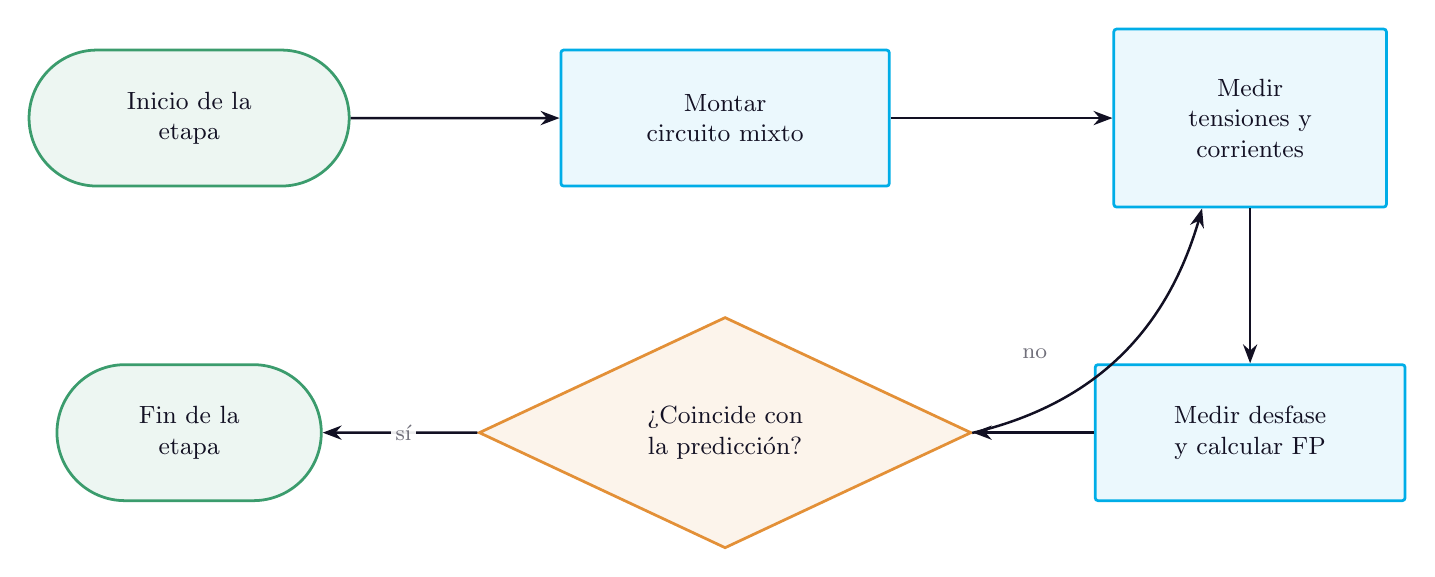
\begin{tikzpicture}[x=1in, y=1in, font=\small]
  % nodos (centro en pulgadas, con el tamano que calcula figuras.py)
  \node[dterminal, minimum width=1.656in, minimum height=0.680in] (n0) at (0.828,-0.445) {Inicio de la \\ etapa};  % ini
  \node[dcaja, minimum width=1.642in, minimum height=0.680in] (n1) at (3.508,-0.445) {Montar \\ circuito mixto};  % a0
  \node[dcaja, minimum width=1.363in, minimum height=0.890in] (n2) at (6.133,-0.445) {Medir \\ tensiones y \\ corrientes};  % a1
  \node[dcaja, minimum width=1.549in, minimum height=0.680in] (n3) at (6.133,-2.018) {Medir desfase \\ y calcular FP};  % a2
  \node[ddecision, minimum width=2.463in, minimum height=1.156in] (n4) at (3.508,-2.018) {\textquestiondown{}Coincide con \\ la predicción?};  % dec
  \node[dterminal, minimum width=1.377in, minimum height=0.680in] (n5) at (0.828,-2.018) {Fin de la \\ etapa};  % fin
  % flechas (las de retorno, curvas)
  \draw[dflecha] (n0) -- (n1);
  \draw[dflecha] (n1) -- (n2);
  \draw[dflecha] (n2) -- (n3);
  \draw[dflecha] (n3) -- (n4);
  \draw[dflecha] (n4) -- (n5);
  \draw[dflecha] (n4) to[bend right=31] (n2);
  % rotulos de las flechas (donde no caen sobre un nodo)
  \node[drotulo] at (1.900,-2.018) {sí};
  \node[drotulo] at (5.056,-1.625) {no};
\end{tikzpicture}
\end{adjustbox}
  \caption{Diagrama de flujo de la etapa 3: Circuito RL mixto}
  \label{fig:flujo-3}
\end{figure}
\begin{pasos}
  \item \textbf{Paso~7:} Montar R1 en serie con el paralelo de R2 y la bobina identificada, con el resistor sensor en serie del lado de tierra, y predecir la corriente, las tensiones y el ángulo con los valores medidos. \emph{(aprox.~\SI{12}{\minute})} \textbf{Comprobación:} La corriente esperada es de unos 8,8 mA con un factor de potencia cercano a 0,95. \textbf{Seguridad:} Montar con el generador apagado.
  \item \textbf{Paso~8:} Medir la corriente total, $V_{R1}$, la tensión del paralelo y las corrientes de rama con el multímetro de verdadero valor eficaz. \emph{(aprox.~\SI{15}{\minute})} \textbf{Comprobación:} Las lecturas deben estar a menos del 2 \% de la predicción. \textbf{Seguridad:} Insertar el amperímetro solo con el circuito desenergizado.
  \item \textbf{Paso~9:} Medir el desfase de la corriente total con el osciloscopio y calcular el factor de potencia $FP = \cos\theta$ y la potencia real $P = V I \cos\theta$ \cite{ref1}. \emph{(aprox.~\SI{8}{\minute})} \textbf{Comprobación:} El ángulo debe estar cerca de 19\textdegree{} de atraso.
\end{pasos}
% --- Etapa 4: Desmontaje y cierre (3 pasos) ---
\subsection{Desmontaje y cierre (\SI{10}{\minute})}\label{sec:etapa-4}
% --- Figura 5: diagrama de flujo de la etapa 4 (TikZ, con la paleta IUB) ---
\begin{figure}[H]
  \centering
\begin{adjustbox}{max width=\linewidth}
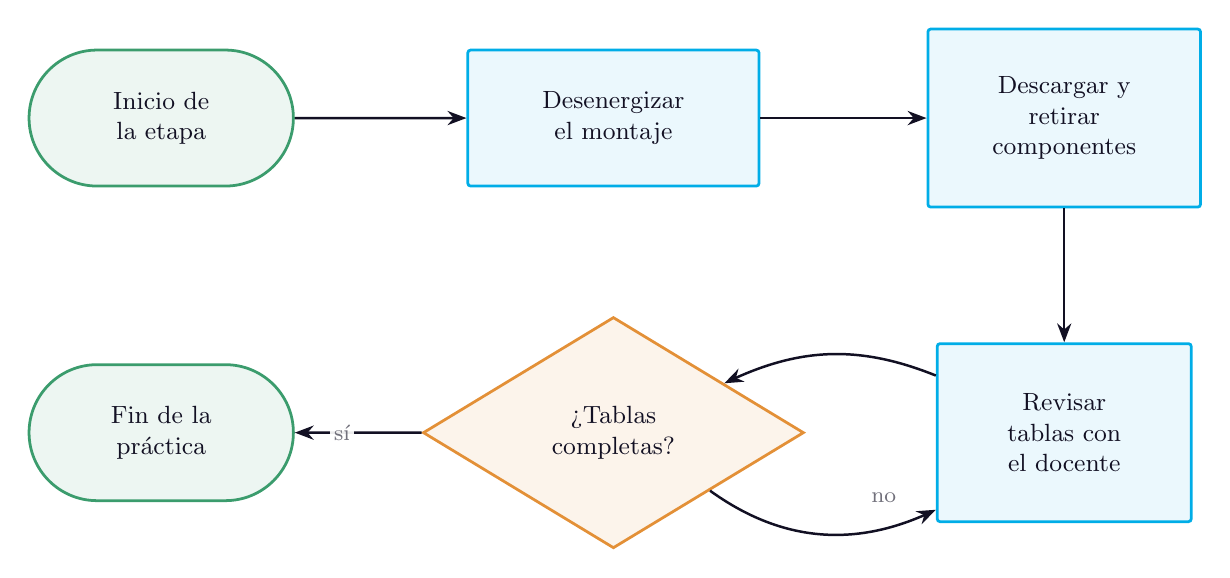
\begin{tikzpicture}[x=1in, y=1in, font=\small]
  % nodos (centro en pulgadas, con el tamano que calcula figuras.py)
  \node[dterminal, minimum width=1.377in, minimum height=0.680in] (n0) at (0.689,-0.445) {Inicio de \\ la etapa};  % ini
  \node[dcaja, minimum width=1.456in, minimum height=0.680in] (n1) at (2.950,-0.445) {Desenergizar \\ el montaje};  % a0
  \node[dcaja, minimum width=1.363in, minimum height=0.890in] (n2) at (5.204,-0.445) {Descargar y \\ retirar \\ componentes};  % a1
  \node[dcaja, minimum width=1.270in, minimum height=0.890in] (n3) at (5.204,-2.018) {Revisar \\ tablas con \\ el docente};  % a2
  \node[ddecision, minimum width=1.905in, minimum height=1.156in] (n4) at (2.950,-2.018) {\textquestiondown{}Tablas \\ completas?};  % dec
  \node[dterminal, minimum width=1.377in, minimum height=0.680in] (n5) at (0.689,-2.018) {Fin de la \\ práctica};  % fin
  % flechas (las de retorno, curvas)
  \draw[dflecha] (n0) -- (n1);
  \draw[dflecha] (n1) -- (n2);
  \draw[dflecha] (n2) -- (n3);
  \draw[dflecha] (n3) to[bend right=24] (n4);
  \draw[dflecha] (n4) -- (n5);
  \draw[dflecha] (n4) to[bend right=31] (n3);
  % rotulos de las flechas (donde no caen sobre un nodo)
  \node[drotulo] at (1.593,-2.018) {sí};
  \node[drotulo] at (4.302,-2.343) {no};
\end{tikzpicture}
\end{adjustbox}
  \caption{Diagrama de flujo de la etapa 4: Desmontaje y cierre}
  \label{fig:flujo-4}
\end{figure}
\begin{pasos}
  \item \textbf{Paso~10:} Apagar el generador de funciones y la fuente, desconectar las puntas del osciloscopio y retirar la alimentación del protoboard. \emph{(aprox.~\SI{3}{\minute})} \textbf{Comprobación:} Ningún indicador de salida debe quedar encendido en el generador ni en la fuente. \textbf{Seguridad:} Desenergizar siempre antes de retirar componentes.
  \item \textbf{Paso~11:} Descargar los condensadores del montaje con la resistencia de descarga, retirar los componentes y devolverlos al kit del grupo con su rótulo. \emph{(aprox.~\SI{4}{\minute})} \textbf{Comprobación:} El kit debe quedar completo, con cada componente en su lugar y con su valor medido anotado.
  \item \textbf{Paso~12:} Revisar con el docente las tablas de registro antes de abandonar el banco. \emph{(aprox.~\SI{3}{\minute})} \textbf{Comprobación:} Las tablas deben estar completas y con unidades; si falta un dato, repetir esa medición antes de desmontar el instrumento.
\end{pasos}

% ---------------------------------------------------------------------
\section{Cuestiones a Resolver}\label{sec:cuestiones}
\begin{enumerate}
  \item \textquestiondown{}Por qué dos métodos independientes, uno en el dominio del tiempo y otro en el de la frecuencia, dan confianza en el valor de la inductancia?
  \item \textquestiondown{}Qué error se cometería al calcular L con la constante de tiempo usando solo la resistencia del resistor y no la de devanado?
  \item \textquestiondown{}A qué valor estándar corresponde la bobina y con qué criterio se eligió?
  \item \textquestiondown{}Qué significa el factor de potencia medido del circuito mixto y cómo podría corregirse?
\end{enumerate}

% ---------------------------------------------------------------------
\section{Análisis de Resultados}\label{sec:analisis}
Calcular la inductancia por los dos métodos, con su diferencia porcentual, e identificar el valor estándar más cercano de la serie de inductores.
\lineablanco
Presentar en la tabla del circuito mixto la predicción, la medición y la diferencia de cada magnitud, y calcular el factor de potencia y las potencias real, reactiva y aparente con las lecturas.
% --- Tabla de registro 1: Inductancia de la bobina sin marcado (2 filas vacías para registrar en el banco) ---
\begin{table}[H]
  \centering
  \caption{Inductancia de la bobina sin marcado}
  \label{tab:registro-1}
  \arrayrulecolor{iubnavy}
  \begin{tabularx}{\linewidth}{>{\raggedright\arraybackslash}X>{\raggedright\arraybackslash}X>{\raggedright\arraybackslash}X>{\raggedright\arraybackslash}X>{\raggedright\arraybackslash}X}
    \rowcolor{iubnavy} \textcolor{white}{\textbf{Método}} & \textcolor{white}{\textbf{Magnitud medida}} & \textcolor{white}{\textbf{Valor medido}} & \textcolor{white}{\textbf{L calculada (mH)}} & \textcolor{white}{\textbf{Diferencia entre métodos (\%)}} \\
    \rule{0pt}{0.8cm} & & & & \\
    \rowcolor{iubfondogris} \rule{0pt}{0.8cm} & & & & \\
    \bottomrule
  \end{tabularx}
\end{table}
% --- Tabla de registro 2: Circuito RL mixto a 10 kHz (7 filas vacías para registrar en el banco) ---
\begin{table}[H]
  \centering
  \caption{Circuito RL mixto a 10 kHz}
  \label{tab:registro-2}
  \arrayrulecolor{iubnavy}
  \begin{tabularx}{\linewidth}{>{\raggedright\arraybackslash}X>{\raggedright\arraybackslash}X>{\raggedright\arraybackslash}X>{\raggedright\arraybackslash}X>{\raggedright\arraybackslash}X}
    \rowcolor{iubnavy} \textcolor{white}{\textbf{Magnitud}} & \textcolor{white}{\textbf{Calculado}} & \textcolor{white}{\textbf{Medido}} & \textcolor{white}{\textbf{Unidad}} & \textcolor{white}{\textbf{Diferencia (\%)}} \\
    \rule{0pt}{0.8cm} & & & & \\
    \rowcolor{iubfondogris} \rule{0pt}{0.8cm} & & & & \\
    \rule{0pt}{0.8cm} & & & & \\
    \rowcolor{iubfondogris} \rule{0pt}{0.8cm} & & & & \\
    \rule{0pt}{0.8cm} & & & & \\
    \rowcolor{iubfondogris} \rule{0pt}{0.8cm} & & & & \\
    \rule{0pt}{0.8cm} & & & & \\
    \bottomrule
  \end{tabularx}
\end{table}

% ---------------------------------------------------------------------
\section{Conclusiones}\label{sec:conclusiones}
Concluir qué inductancia tiene la bobina y a qué valor estándar corresponde, apoyándose en la concordancia de los dos métodos, y si el circuito mixto se comporta como predice el cálculo; relacionar la práctica con los criterios de medición en circuitos resistivos, inductivos y RL del RA.
\lineablanco
\begin{itemize}
  \item \textquestiondown{}Qué método resultó más preciso y por qué?
  \item \textquestiondown{}Qué aprendieron sobre la medición de inductancia sin un medidor LCR?
  \item \textquestiondown{}Hubo algún resultado inesperado en el circuito mixto?
\end{itemize}

% ---------------------------------------------------------------------
\section{Recomendaciones de Seguridad}\label{sec:seguridad}
\begin{itemize}
  \item Conectar las tierras de las dos puntas del osciloscopio a un mismo nodo de referencia: unirlas a nodos distintos cortocircuita el elemento que queda entre ellas.
  \item Insertar el amperímetro en serie con la rama solo con el circuito desenergizado y con el instrumento en la función y la escala de corriente; nunca conectarlo en paralelo con la fuente.
  \item No interrumpir bruscamente la corriente de la bobina con el circuito energizado.
  \item Desenergizar antes de pasar del montaje de los métodos 1 y 2 al circuito mixto.
\end{itemize}

% ---------------------------------------------------------------------
\section{Bibliografía}\label{sec:bibliografia}
% Las fuentes cargadas se citan en el texto con \cite{refN}; el \nocite del principio fija su orden y \nocite{*} incluye las demás del .bib.
\nocite{*}
\bibliografia

\end{document}
